%\documentstyle[epsf,twocolumn]{jarticle}       %LaTeX2e仕様
%\documentclass[twocolumn]{jarticle}     %pLaTeX2e仕様(platex.exeの場合)
\documentclass[onecolumn]{ujarticle}   %pLaTeX2e仕様(uplatex.exeの場合)
%%%%%%%%%%%%%%%%%%%%%%%%%%%%%%%%%%%%%%%%%%%%%%%%%%%%%%%%%%%%%%
%%
%%  基本バージョン
%%
%%%%%%%%%%%%%%%%%%%%%%%%%%%%%%%%%%%%%%%%%%%%%%%%%%%%%%%%%%%%%%%%
\setlength{\topmargin}{-45pt}
%\setlength{\oddsidemargin}{0cm}
\setlength{\oddsidemargin}{-7.5mm}
%\setlength{\evensidemargin}{0cm}
\setlength{\textheight}{24.1cm}
%setlength{\textheight}{25cm}
\setlength{\textwidth}{17.4cm}
%\setlength{\textwidth}{172mm}
\setlength{\columnsep}{11mm}

%\kanjiskip=.07zw plus.5pt minus.5pt


% 【節が変わるごとに (1.1)(1.2) … (2.1)(2.2) と数式番号をつけるとき】
%\makeatletter
%\renewcommand{\theequation}{%
%\thesection.\arabic{equation}} %\@addtoreset{equation}{section}
%\makeatother

%\renewcommand{\arraystretch}{0.95} 行間の設定
%%%%%%%%%%%%%%%%%%%%%%%%%%%%%%%%%%%%%%%%%%%%%%%%%%%%%%%%
%\usepackage{graphicx}   %pLaTeX2e仕様(\documentstyle ->\documentclass)
\usepackage[dvipdfmx]{graphicx}
\usepackage{subcaption}
\usepackage{multirow}
\usepackage{amsmath}
\usepackage{url}
\usepackage{ulem}
%%%%%%%%%%%%%%%%%%%%%%%%%%%%%%%%%%%%%%%%%%%%%%%%%%%%%%%%
\begin{document}

	%bibtex用の設定
	%\bibliographystyle{ujarticle}
	\noindent

	\hspace{1em}
	2019 年 12 月 13 日
	ゼミ資料
	\hfill
	M1 寺内 光

	\vspace{2mm}

	\hrule

	\begin{center}
		{\Large \bf 進捗報告}
	\end{center}


	\hrule
	\vspace{3mm}

	% ‚ここから 文章 Start!
	\section{今週やったこと}
	\begin{itemize}{
		\item{PyTorchベースのDeepLab(PSPNet)の改良調査}
		\item{データラベルの整形}
	}
	\end{itemize}

	\subsection{PyTorchベースのDeepLab(PSPNet)の改良調査}
	今週はPyTorchのモデルの精度が出ない理由の調査を進めた.同じようにベンチマークの精度が出ないというissueを上げている人がいたのでその改善策に従ってバッチサイズを変えたりパラメータ調整をしてみたが(少しは上がったものの)あまり効果はなかった.再現実験をしているのに精度が出ないのは未だに謎であり,まだ解決はされていない.
	また,レポジトリの作者が公開している PSPNet のモデルチェックポイントを用いて Pascal VOC データセットで学習したところ,validation {\it mIoU} は約82%となり,Tensorflow ベースの DeepLab と同等の精度が出た.この重みを 4 コマで試してみたいと思っているが,チェックポイントがモデル構造も記憶しているために出力の整合が合わないためにそのまま用いることができない.おそらく途中の出力を取ってくることはできると思うので,方法を探りながら試したい.
	一応このレポジトリで DeepLab と PSPNet の比較とFocal loss があまり効いてこなかったということの検証ができたのでそれで収めておくのが丸いかもしれない...

	\subsection{データラベルの整形}
	後期発表の時点で,口の中がラベルとして認識されていない,ノイズののったデータがある,萌えタッチで頬に目のラベルがついている等の問題点がいくつかあったため,photo shopで整形した.
	図 \ref{fig:fix_figure} に整形例を示す.現在,このラベル修正を加えた {\it mIoU} の変化を見るために実験を回している.
	\begin{figure}[h]
		\centering
		\vspace{-7mm}
		\begin{subfigure}{0.45\columnwidth}
			\centering
			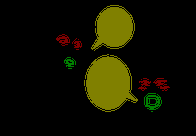
\includegraphics[width=1.0\columnwidth]{before_mouth.png}
			\caption{修正前}
		\end{subfigure}
		\begin{subfigure}{0.45\columnwidth}
			\centering
			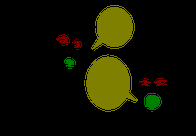
\includegraphics[width=1.0\columnwidth]{after_mouth.png}
			\caption{修正後}
		\end{subfigure}
		\begin{subfigure}{0.45\columnwidth}
			\centering
			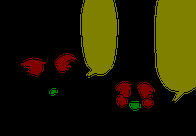
\includegraphics[width=1.0\columnwidth]{before_cheek.png}
			\caption{修正前}
		\end{subfigure}
		\begin{subfigure}{0.45\columnwidth}
			\centering
			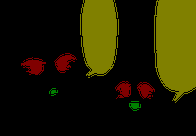
\includegraphics[width=1.0\columnwidth]{after_cheek.png}
			\caption{修正後}
		\end{subfigure}
		\caption{修正前ラベルと修正後ラベル}
		\label{fig:fix_figure}
	\end{figure}

	\section{年内の方針}
	年内に残りのAuto-Labを試して年明けからは新しいタスクを設定したいと考えている.


\end{document}
